\documentclass[12pt]{article}
\usepackage[table]{xcolor}
\usepackage[shortlabels]{enumitem}
\usepackage{tabularx,xltabular}
\usepackage{graphicx}
\usepackage{hyperref}
\usepackage{verbatim}
\usepackage{geometry}
\usepackage{ulem}
\usepackage[official]{eurosym}
\usepackage{tikz}
\usetikzlibrary{arrows,backgrounds,calc,decorations.markings,patterns,3d,positioning,fit,angles, quotes}
\usepackage{pgfplots}
\pgfplotsset{compat = newest}
\usetikzlibrary{fit}
\newcommand\addvmargin[1]{
\usetikzlibrary{arrows}
\node[fit=(current bounding box),inner ysep=#1,inner xsep=0]{};}
\usepackage{cancel}
\usepackage{fontspec}
\usepackage{array}  
\geometry{a4paper, top=2cm, left=2cm, right=2cm, bottom=2cm, headsep=1cm}
\usepackage{tabu}
\usepackage{pst-node}
\usepackage{colortbl}
\usepackage{array}
\usepackage{german}
\setlength\parindent{0pt}
\newcolumntype{?}{!{\vrule width 1pt}}
\usepackage{makecell}
\usepackage{pbox}
\usepackage{amssymb}
\usepackage{amsmath}
\usepackage{booktabs}
\newcolumntype{L}[1]{>{\raggedright\let\newline\\\arraybackslash\hspace{0pt}}m{#1}}
\newcolumntype{C}[1]{>{\centering\let\newline\\\arraybackslash\hspace{0pt}}m{#1}}
\newcolumntype{R}[1]{>{\raggedleft\let\newline\\\arraybackslash\hspace{0pt}}m{#1}}
\begin{document}
\rightline{}
\centerline{{\Large }} 
\vspace{1cm}
\noindent \\


\begin{tabularx}{\textwidth}{|C{1.0cm}|X|}
\arrayrulecolor{black}\hline
a)&{\pbox{5cm}{
\tikzstyle{background grid}=[draw, black!15,step=.5cm]
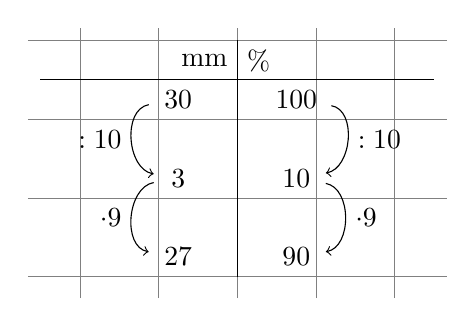
\begin{tikzpicture}[show background grid]
\draw[black] (0cm,0cm) -- (0cm,-3cm); 
\draw[black] (-2.5 cm,-0.5cm) -- (2.5cm,-0.5cm); 
\node[left] at (0 cm,-0.25cm) {mm};
\node[right] at (0 cm,-0.255cm) {\%};
\node[circle] (1) at (-0.75 cm,-0.75cm) {30};
\node[circle] (2) at (-0.75 cm,-1.75cm) {3};
\node[circle] (3) at (-0.75 cm,-2.75cm) {27};
\node[circle] (4) at (0.75 cm,-0.75cm) {100};
\node[circle] (5) at (0.75 cm,-1.75cm) {10};
\node[circle] (6) at (0.75 cm,-2.75cm) {90};
\draw[->] (1) to [out=190,in=170] node[left] {$:10$}  (2) ;
\draw[->] (2) to [out=190,in=170] node[left] {$\cdot 9$}  (3) ;
\draw[->] (4) to [out=350,in=10] node[right] {$:10$}  (5) ;
\draw[->] (5) to [out=350,in=10] node[right] {$\cdot9$}  (6) ;
\end{tikzpicture}
\newline
Oder: \newline
Gesamtlänge: 30\,mm, Länge der Schraffur: 27\,mm. Das bedeutet: \newline
$\frac{27}{30}=0,9=90\%$
}}
\\\hline
\end{tabularx}
\vspace{0.5cm}
\begin{tabularx}{\textwidth}{|C{1.0cm}|X|}
\arrayrulecolor{black}\hline
b)&{\pbox{5cm}{
\tikzstyle{background grid}=[draw, black!15,step=.5cm]
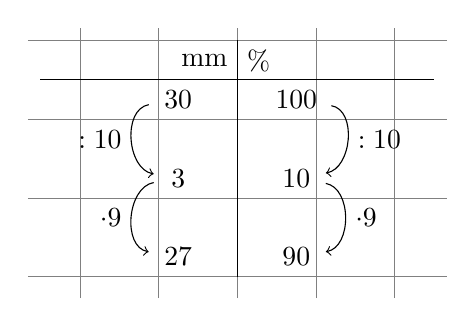
\begin{tikzpicture}[show background grid]
\draw[black] (0cm,0cm) -- (0cm,-3cm); 
\draw[black] (-2.5 cm,-0.5cm) -- (2.5cm,-0.5cm); 
\node[left] at (0 cm,-0.25cm) {mm};
\node[right] at (0 cm,-0.255cm) {\%};
\node[circle] (1) at (-0.75 cm,-0.75cm) {30};
\node[circle] (2) at (-0.75 cm,-1.75cm) {3};
\node[circle] (3) at (-0.75 cm,-2.75cm) {27};
\node[circle] (4) at (0.75 cm,-0.75cm) {100};
\node[circle] (5) at (0.75 cm,-1.75cm) {10};
\node[circle] (6) at (0.75 cm,-2.75cm) {90};
\draw[->] (1) to [out=190,in=170] node[left] {$:10$}  (2) ;
\draw[->] (2) to [out=190,in=170] node[left] {$\cdot 9$}  (3) ;
\draw[->] (4) to [out=350,in=10] node[right] {$:10$}  (5) ;
\draw[->] (5) to [out=350,in=10] node[right] {$\cdot9$}  (6) ;
\end{tikzpicture}
\newline
Oder: \newline
Gesamtlänge: 30\,mm, Länge der Schraffur: 27\,mm. Das bedeutet: \newline
$\frac{27}{30}=0,9=90\%$
}}
\\\hline
\end{tabularx}
\vspace{0.5cm}
\begin{tabularx}{\textwidth}{|C{1.0cm}|X|}
\arrayrulecolor{black}\hline
a)&{
\begingroup\setlength{\jot}{0.02cm}
\tikzstyle{background grid}=[draw, black!15,step=.5cm]
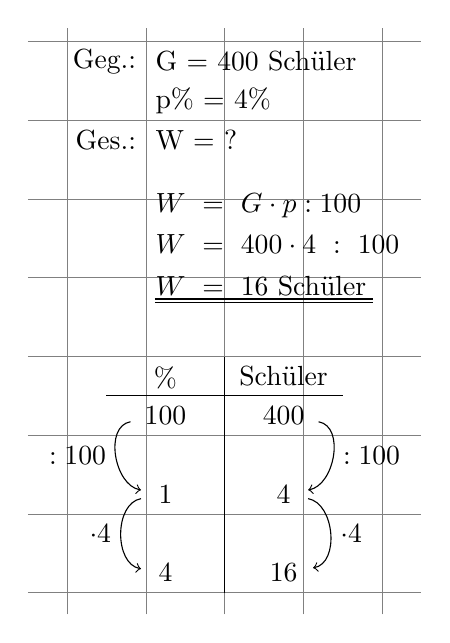
\begin{tikzpicture}[show background grid]
\node[left] at (0,-0.25) {Geg.: };
\node[right] at (0,-0.25) {G = 400 Schüler};
\node[right] at (0,-0.75) {p\% = 4\%};
\node[left] at (0,-1.-0.25) {Ges.: };
\node[right] at (0,-1.-0.25) {W  = ? };
\node[below right] at (0,-1.75) {
$\begin{aligned}
W\ &=\ G\cdot p : 100 \\
W\ &=\ 400\cdot 4\ :\ 100 \\
\makebox[0pt][l]{\uuline{\phantom{W\%\ =\ 16\ \mbox{Schüler}}}}
W\ &=\ 16\ \mbox{Schüler}
\end{aligned}$};

\draw[black] (1cm,-4cm) -- (1cm,-7cm); 
\draw[black] (-0.5 cm,-4.5cm) -- (2.5cm,-4.5cm); 
\node[below] at (0.25 cm,-4cm) {\%};
\node[below] at  (1.75 cm,-4cm) {Schüler};
\node[circle] (1) at (0.25 cm,-4.75cm) {100};
\node[circle] (2) at (0.25 cm,-5.75cm) {1};
\node[circle] (3) at (0.25 cm,-6.75cm) {4};
\node[circle] (4) at (1.75 cm,-4.75cm) {400};
\node[circle] (5) at (1.75 cm,-5.75cm) {4};
\node[circle] (6) at (1.75 cm,-6.75cm) {16};
\draw[->] (1) to [out=190,in=170] node[left] {$:100$}  (2) ;
\draw[->] (2) to [out=190,in=170] node[left] {$\cdot 4$}  (3) ;
\draw[->] (4) to [out=350,in=10] node[right] {$:100$}  (5) ;
\draw[->] (5) to [out=350,in=10] node[right] {$\cdot4$}  (6) ;
\end{tikzpicture}
\endgroup}
\\\hline
\end{tabularx}
\vspace{0.5cm}
\begin{tabularx}{\textwidth}{|C{1.0cm}|X|}
\arrayrulecolor{black}\hline
a)&{
\begingroup\setlength{\jot}{0.02cm}
\tikzstyle{background grid}=[draw, black!15,step=.5cm]
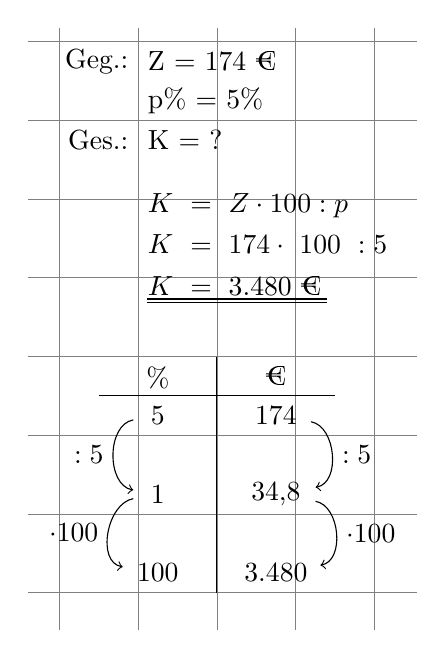
\begin{tikzpicture}[show background grid]
\node[left] at (0,-0.25) {Geg.: };
\node[right] at (0,-0.25) {Z = 174 €};
\node[right] at (0,-0.75) {p\% = 5\%};
\node[left] at (0,-1.-0.25) {Ges.: };
\node[right] at (0,-1.-0.25) {K  = ? };
\node[below right] at (0,-1.75) {
$\begin{aligned}
K\ &=\ Z\cdot 100 : p \\
K\ &=\ 174\cdot\ 100\ :5 \\
\makebox[0pt][l]{\uuline{\phantom{G\%\ =\ 3.480\ \mbox{€}}}}
K\ &=\ 3.480\ \mbox{€}
\end{aligned}$};

\draw[black] (1cm,-4cm) -- (1cm,-7cm); 
\draw[black] (-0.5 cm,-4.5cm) -- (2.5cm,-4.5cm); 
\node[below] at (0.25 cm,-4cm) {\%};
\node[below] at  (1.75 cm,-4cm) {€};
\node[circle] (1) at (0.25 cm,-4.75cm) {5};
\node[circle] (2) at (0.25 cm,-5.75cm) {1};
\node[circle] (3) at (0.25 cm,-6.75cm) {100};
\node[circle] (4) at (1.75 cm,-4.75cm) {174};
\node[circle] (5) at (1.75 cm,-5.75cm) {34,8};
\node[circle] (6) at (1.75 cm,-6.75cm) {3.480};
\draw[->] (1) to [out=190,in=170] node[left] {$:5$}  (2) ;
\draw[->] (2) to [out=190,in=170] node[left] {$\cdot 100$}  (3) ;
\draw[->] (4) to [out=350,in=10] node[right] {$:5$}  (5) ;
\draw[->] (5) to [out=350,in=10] node[right] {$\cdot100$}  (6) ;
\end{tikzpicture}
\endgroup}
\\\hline
\end{tabularx}
\vspace{0.5cm}
\begin{tabularx}{\textwidth}{|C{1.0cm}|X|}
\arrayrulecolor{black}\hline
a)&{
\pbox{5cm}{
$\begin{aligned}
geg.: K&=3.800 € \\
   p\%&=5 \% \\
ges.: Z_{5M}&=? \\
 Z&=K\cdot p\% \\
 Z&=3.800\cdot 0,05 \\
 Z&=190 €\\
 Z_{1M}&=190 € : 12\\
 Z_{1M}&=15,83 €\\
 Z_{5M}&=15,83 € \cdot 5\\
\makebox[0pt][l]{\uuline{\phantom{$ Z_{5M}=79,17 €\\$} } }
 Z_{5M}&=79,17 €\\
\end{aligned}$ \\
}}
\\\hline
\end{tabularx}
\vspace{0.5cm}
\begin{tabularx}{\textwidth}{|C{1.0cm}|X|}
\arrayrulecolor{black}\hline
a)&{
\begingroup\setlength{\jot}{0.02cm}
\tikzstyle{background grid}=[draw, black!15,step=.5cm]
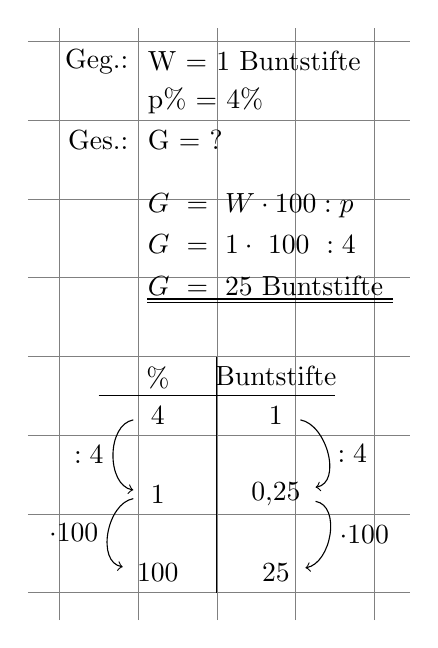
\begin{tikzpicture}[show background grid]
\node[left] at (0,-0.25) {Geg.: };
\node[right] at (0,-0.25) {W = 1 Buntstifte};
\node[right] at (0,-0.75) {p\% = 4\%};
\node[left] at (0,-1.-0.25) {Ges.: };
\node[right] at (0,-1.-0.25) {G  = ? };
\node[below right] at (0,-1.75) {
$\begin{aligned}
G\ &=\ W\cdot 100 : p \\
G\ &=\ 1\cdot\ 100\ :4 \\
\makebox[0pt][l]{\uuline{\phantom{G\%\ =\ 25\ \mbox{Buntstifte}}}}
G\ &=\ 25\ \mbox{Buntstifte}
\end{aligned}$};

\draw[black] (1cm,-4cm) -- (1cm,-7cm); 
\draw[black] (-0.5 cm,-4.5cm) -- (2.5cm,-4.5cm); 
\node[below] at (0.25 cm,-4cm) {\%};
\node[below] at  (1.75 cm,-4cm) {Buntstifte};
\node[circle] (1) at (0.25 cm,-4.75cm) {4};
\node[circle] (2) at (0.25 cm,-5.75cm) {1};
\node[circle] (3) at (0.25 cm,-6.75cm) {100};
\node[circle] (4) at (1.75 cm,-4.75cm) {1};
\node[circle] (5) at (1.75 cm,-5.75cm) {0,25};
\node[circle] (6) at (1.75 cm,-6.75cm) {25};
\draw[->] (1) to [out=190,in=170] node[left] {$:4$}  (2) ;
\draw[->] (2) to [out=190,in=170] node[left] {$\cdot 100$}  (3) ;
\draw[->] (4) to [out=350,in=10] node[right] {$:4$}  (5) ;
\draw[->] (5) to [out=350,in=10] node[right] {$\cdot100$}  (6) ;
\end{tikzpicture}
\endgroup}
\\\hline
\end{tabularx}
\vspace{0.5cm}
\begin{tabularx}{\textwidth}{|C{1.0cm}|X|}
\arrayrulecolor{black}\hline
a)&{
\begingroup\setlength{\jot}{0.02cm}
\tikzstyle{background grid}=[draw, black!15,step=.5cm]
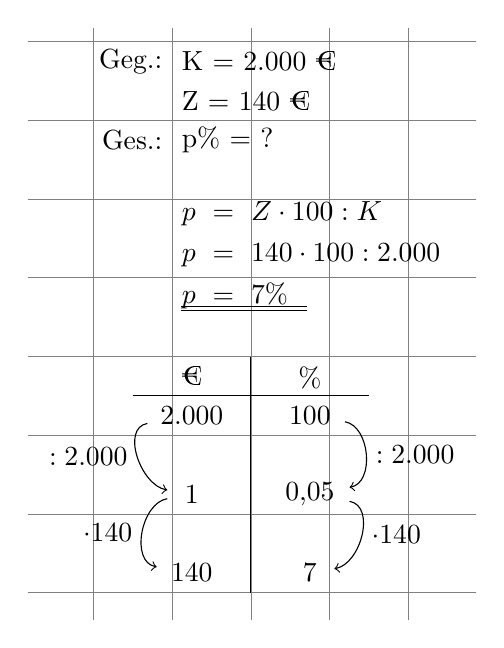
\begin{tikzpicture}[show background grid]
\node[left] at (0,-0.25) {Geg.: };
\node[right] at (0,-0.25) {K = 2.000 €};
\node[right] at (0,-0.75) {Z = 140 €};
\node[left] at (0,-1.25) {Ges.: };
\node[right] at (0,-1.25) {p\%  = ? };
\node[below right] at (0,-1.85) {
$\begin{aligned}
p\ &=\ Z\cdot 100 : K \\
p\ &=\ 140\cdot 100 : 2.000\ \\
\makebox[0pt][l]{\uuline{\phantom{p\%\ =\ 7\% }}}
p\ &=\ 7\% 
\end{aligned}$};

\draw[black] (1cm,-4cm) -- (1cm,-7cm); 
\draw[black] (-0.5 cm,-4.5cm) -- (2.5cm,-4.5cm); 
\node[below] at (0.25 cm,-4cm) {€};
\node[below] at  (1.75 cm,-4cm) {\%};
\node[circle] (1) at (0.25 cm,-4.75cm) {2.000};
\node[circle] (2) at (0.25 cm,-5.75cm) {1};
\node[circle] (3) at (0.25 cm,-6.75cm) {140};
\node[circle] (4) at (1.75 cm,-4.75cm) {100};
\node[circle] (5) at (1.75 cm,-5.75cm) {0,05};
\node[circle] (6) at (1.75 cm,-6.75cm) {7};
\draw[->] (1) to [out=190,in=170] node[left] {$:2.000$}  (2) ;
\draw[->] (2) to [out=190,in=170] node[left] {$\cdot 140$}  (3) ;
\draw[->] (4) to [out=350,in=10] node[right] {$:2.000$}  (5) ;
\draw[->] (5) to [out=350,in=10] node[right] {$\cdot140$}  (6) ;
\end{tikzpicture}
\endgroup}
\\\hline
\end{tabularx}
\vspace{0.5cm}
\begin{tabularx}{\textwidth}{|C{1.0cm}|X|}
\arrayrulecolor{black}\hline
a)&{
\begingroup\setlength{\jot}{0.02cm}
\tikzstyle{background grid}=[draw, black!15,step=.5cm]
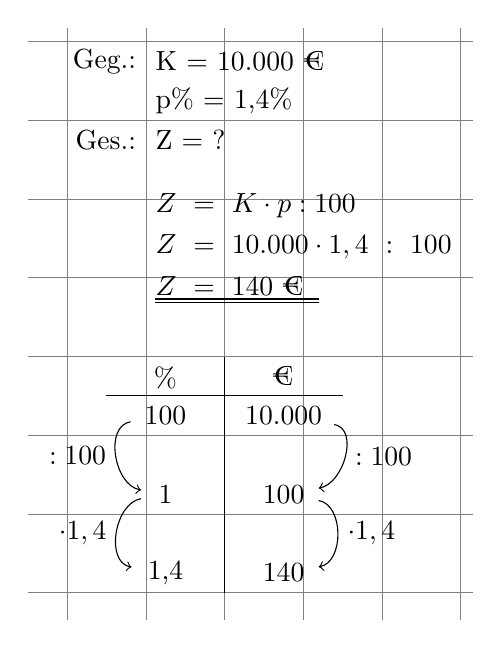
\begin{tikzpicture}[show background grid]
\node[left] at (0,-0.25) {Geg.: };
\node[right] at (0,-0.25) {K = 10.000 €};
\node[right] at (0,-0.75) {p\% = 1,4\%};
\node[left] at (0,-1.-0.25) {Ges.: };
\node[right] at (0,-1.-0.25) {Z  = ? };
\node[below right] at (0,-1.75) {
$\begin{aligned}
Z\ &=\ K\cdot p : 100 \\
Z\ &=\ 10.000\cdot 1,4\ :\ 100 \\
\makebox[0pt][l]{\uuline{\phantom{W\%\ =\ 140\ \mbox{€}}}}
Z\ &=\ 140\ \mbox{€}
\end{aligned}$};

\draw[black] (1cm,-4cm) -- (1cm,-7cm); 
\draw[black] (-0.5 cm,-4.5cm) -- (2.5cm,-4.5cm); 
\node[below] at (0.25 cm,-4cm) {\%};
\node[below] at  (1.75 cm,-4cm) {€};
\node[circle] (1) at (0.25 cm,-4.75cm) {100};
\node[circle] (2) at (0.25 cm,-5.75cm) {1};
\node[circle] (3) at (0.25 cm,-6.75cm) {1,4};
\node[circle] (4) at (1.75 cm,-4.75cm) {10.000};
\node[circle] (5) at (1.75 cm,-5.75cm) {100};
\node[circle] (6) at (1.75 cm,-6.75cm) {140};
\draw[->] (1) to [out=190,in=170] node[left] {$:100$}  (2) ;
\draw[->] (2) to [out=190,in=170] node[left] {$\cdot 1,4$}  (3) ;
\draw[->] (4) to [out=350,in=10] node[right] {$:100$}  (5) ;
\draw[->] (5) to [out=350,in=10] node[right] {$\cdot1,4$}  (6) ;
\end{tikzpicture}
\endgroup}
\\\hline
\end{tabularx}
\vspace{0.5cm}
\begin{tabularx}{\textwidth}{|C{1.0cm}|X|}
\arrayrulecolor{black}\hline
a)&{$$\frac{2}{3}=0,67=66,67\%$$}
\\\hline
\end{tabularx}
\vspace{0.5cm}
\begin{tabularx}{\textwidth}{|C{1.0cm}|X|}
\arrayrulecolor{black}\hline
b)&{$$\frac{1}{2}=0,5=50\%$$}
\\\hline
\end{tabularx}
\vspace{0.5cm}
\begin{tabularx}{\textwidth}{|C{1.0cm}|X|}
\arrayrulecolor{black}\hline
a)&{
\begingroup\setlength{\jot}{0.02cm}
\tikzstyle{background grid}=[draw, black!15,step=.5cm]
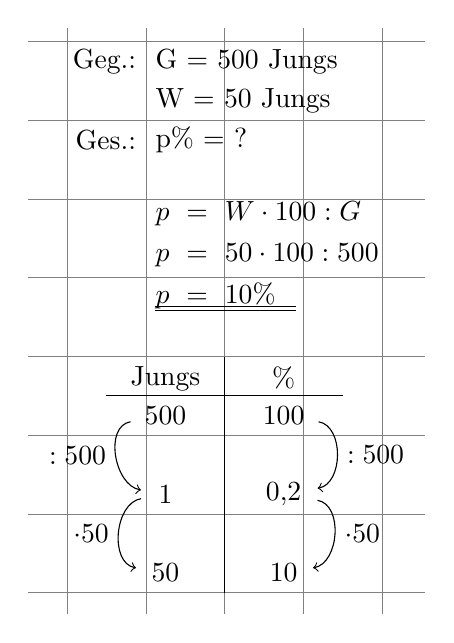
\begin{tikzpicture}[show background grid]
\node[left] at (0,-0.25) {Geg.: };
\node[right] at (0,-0.25) {G = 500 Jungs};
\node[right] at (0,-0.75) {W = 50 Jungs};
\node[left] at (0,-1.25) {Ges.: };
\node[right] at (0,-1.25) {p\%  = ? };
\node[below right] at (0,-1.85) {
$\begin{aligned}
p\ &=\ W\cdot 100 : G \\
p\ &=\ 50\cdot 100 : 500\ \\
\makebox[0pt][l]{\uuline{\phantom{p\%\ =\ 10\% }}}
p\ &=\ 10\% 
\end{aligned}$};

\draw[black] (1cm,-4cm) -- (1cm,-7cm); 
\draw[black] (-0.5 cm,-4.5cm) -- (2.5cm,-4.5cm); 
\node[below] at (0.25 cm,-4cm) {Jungs};
\node[below] at  (1.75 cm,-4cm) {\%};
\node[circle] (1) at (0.25 cm,-4.75cm) {500};
\node[circle] (2) at (0.25 cm,-5.75cm) {1};
\node[circle] (3) at (0.25 cm,-6.75cm) {50};
\node[circle] (4) at (1.75 cm,-4.75cm) {100};
\node[circle] (5) at (1.75 cm,-5.75cm) {0,2};
\node[circle] (6) at (1.75 cm,-6.75cm) {10};
\draw[->] (1) to [out=190,in=170] node[left] {$:500$}  (2) ;
\draw[->] (2) to [out=190,in=170] node[left] {$\cdot 50$}  (3) ;
\draw[->] (4) to [out=350,in=10] node[right] {$:500$}  (5) ;
\draw[->] (5) to [out=350,in=10] node[right] {$\cdot50$}  (6) ;
\end{tikzpicture}
\endgroup}
\\\hline
\end{tabularx}
\vspace{0.5cm}
\begin{tabularx}{\textwidth}{|C{1.0cm}|X|}
\arrayrulecolor{black}\hline
a)&{\pbox{15cm}{
Nach 1 Jahren: \\
$\begin{aligned}
Z_1&=K_{start}\cdot p\% \\
&=7.250 € \cdot 0,04 \\
&=290 €\\
K_1&=K_{start}+Z \\
&=7.250 €+ 290 €\\
\makebox[0pt][l]{\uuline{\phantom{$K_1=7.540 €\\$} } }
K_1&=7.540 €\\
\end{aligned}$ \\
Nach 2 Jahren: \\
$\begin{aligned}
Z_2&=K_1\cdot p\% \\
&=7.540 € \cdot 0,04 \\
&=301,6 €\\
K_2&=K_1+Z \\
&=7.540 €+ 301,6 €\\
\makebox[0pt][l]{\uuline{\phantom{$K_2=7.841,6 €\\$} } }
K_2&=7.841,6 €\\
\end{aligned}$ \\
}}
\\\hline
\end{tabularx}
\vspace{0.5cm}
\begin{tabularx}{\textwidth}{|C{1.0cm}|X|}
\arrayrulecolor{black}\hline
\end{tabularx}
\vspace{0.5cm}
\end{document}